% 附录 AA：替代位形——仿星器、球形托卡马克与场反位形（v1.25.0 新增）
% 数值唯一来源：tools/calc/appAA_calc.py -> tools/calc/appAA_calc.txt（正文数字的唯一来源；检查项 P32）
% 单位写法：T / MA / Pa / m^-3 / s / %，全部走 \mathrm{}，不放中文字符进数学字体。
% 版权口径：只借鉴经典教材与文献的物理结论、公式形式与题型；文字、数值与表格自拟并独立复算。
% 本书不列 DOI，只给书名、作者、年份、卷期页。
% 分工：M–Z 讲的是托卡马克这一条主线（加热、边界、约束、增益、破裂、快粒子、辐射、强场、堆工程）；
%       本附录跳出主线，讲三种「不走托卡马克路」的位形，以及它们各自付出的代价。

\section{三种位形的一张地图}
\label{sec:app-aa-map}

托卡马克用环向场加等离子体电流产生极向场，把磁力线拧成螺旋。
三种替代方案走别的路：\textbf{仿星器}（螺旋线圈直接造出旋转变换，
不需要等离子体电流）、\textbf{球形托卡马克}（把环径比压到接近 $1$）、
\textbf{场反位形}（连环向场都不要，$\beta$ 直接顶到 $1$）。

第一步是把它们放在同一张地图上。位形的几何由一个数决定：环径比
\begin{equation}
A = \frac{R}{a},
\label{eq:app-aa-eps}
\end{equation}
反过来说，逆环径比 $\varepsilon = a/R$ 就是「环有多胖」：
\begin{equation}
\varepsilon = \frac{1}{A}.
\label{eq:app-aa-epsnum}
\end{equation}
D1 托卡马克取 $A=3.1$（$\varepsilon = 0.32258$）、球形托卡马克取 $A=1.5$
（$\varepsilon = 0.66667$）、仿星器取 $A=10.377$（$\varepsilon = 0.096364$）。
\textbf{三个位形的 $\varepsilon$ 相差近七倍}。后面所有差别几乎都从这里长出来。

第二个数是等离子体压强与磁压之比：
\begin{equation}
\beta = \frac{2\mu_0 p}{B^2},\qquad p = n\,k_BT,
\label{eq:app-aa-beta}
\end{equation}
以及工程上更常用的归一化比压
\begin{equation}
\beta_N = \beta\,[\%]\cdot\frac{a\,[\mathrm{m}]\,B\,[\mathrm{T}]}{I_p\,[\mathrm{MA}]}.
\label{eq:app-aa-betan}
\end{equation}
代入三组参数（$n$、$T$、$B$、$I_p$ 全部在脚本的声明段里）：
D1 的 $\beta = 1.318\%$（$\beta_N = 1.5523$）、
球形托卡马克的 $\beta = 4.027\%$（$\beta_N = 1.2483$）、
仿星器的 $\beta = 1.031\%$（$\beta_N = 1.3659$，仿星器没有环向电流，这里用 $1\ \mathrm{MA}$ 只为给出量级对照）。
\textbf{球形托卡马克的 $\beta$ 是 D1 的 $3.0553$ 倍}，而两者的 $\beta_N$ 却差不多，
说明\textbf{$\beta_N$ 才是跨装置可比的标尺}。

\begin{table}[htbp]
\centering
\small
\caption{三种位形的一张地图。最后一行是关键差别：
\textbf{仿星器不需要等离子体电流}，于是没有电流驱动、没有破裂、也没有电流剖面要管。}
\label{tab:app-aa-map}
\begin{tabular}{p{3.0cm}p{3.2cm}p{3.2cm}p{3.5cm}}
\toprule
量 & D1 托卡马克 & 球形托卡马克 & 仿星器 \\
\midrule
环径比 $A=R/a$ & $3.1$ & $1.5$ & $10.377$ \\
逆环径比 $\varepsilon$ & $0.32258$ & $0.66667$ & $0.096364$ \\
压强 $p$ & $1.473\times10^{5}\ \mathrm{Pa}$ & $16022\ \mathrm{Pa}$ & $25635\ \mathrm{Pa}$ \\
比压 $\beta$ & $1.318\%$ & $4.027\%$ & $1.031\%$ \\
归一化比压 $\beta_N$ & $1.5523$ & $1.2483$ & $1.3659$ \\
环向电流 & 有（$9\ \mathrm{MA}$） & 有（$2\ \mathrm{MA}$） & \textbf{没有} \\
\bottomrule
\end{tabular}

\end{table}

\begin{tip}{先问「它拿什么换什么」}{tip-app-aa-map}
替代位形没有「更好」的，只有「换」的：仿星器用\textbf{三维线圈的工程复杂度}换掉了等离子体电流；
球形托卡马克用\textbf{中心柱的空间}换来了高 $\beta$；场反位形用\textbf{稳定性}换来了 $\beta=1$。
一旦代价能算出来，就知道该往哪里优化。
\end{tip}

{\footnotesize
\textbf{出处：}三种位形的分类与环径比、比压的定义参照 Freidberg
\emph{Ideal Magnetohydrodynamics}（1987，第 1 章）与 Wesson \emph{Tokamaks}
（第 4 版，2011，第 1 章）。
球形托卡马克与仿星器的量级取自各自的装置手册
（NSTX-U 与 W7-X，只给装置名与量级）。本节数字由
\texttt{tools/\allowbreak{}calc/\allowbreak{}appAA\_calc.py} 复算。
}

\begin{figure}[htbp]
\centering
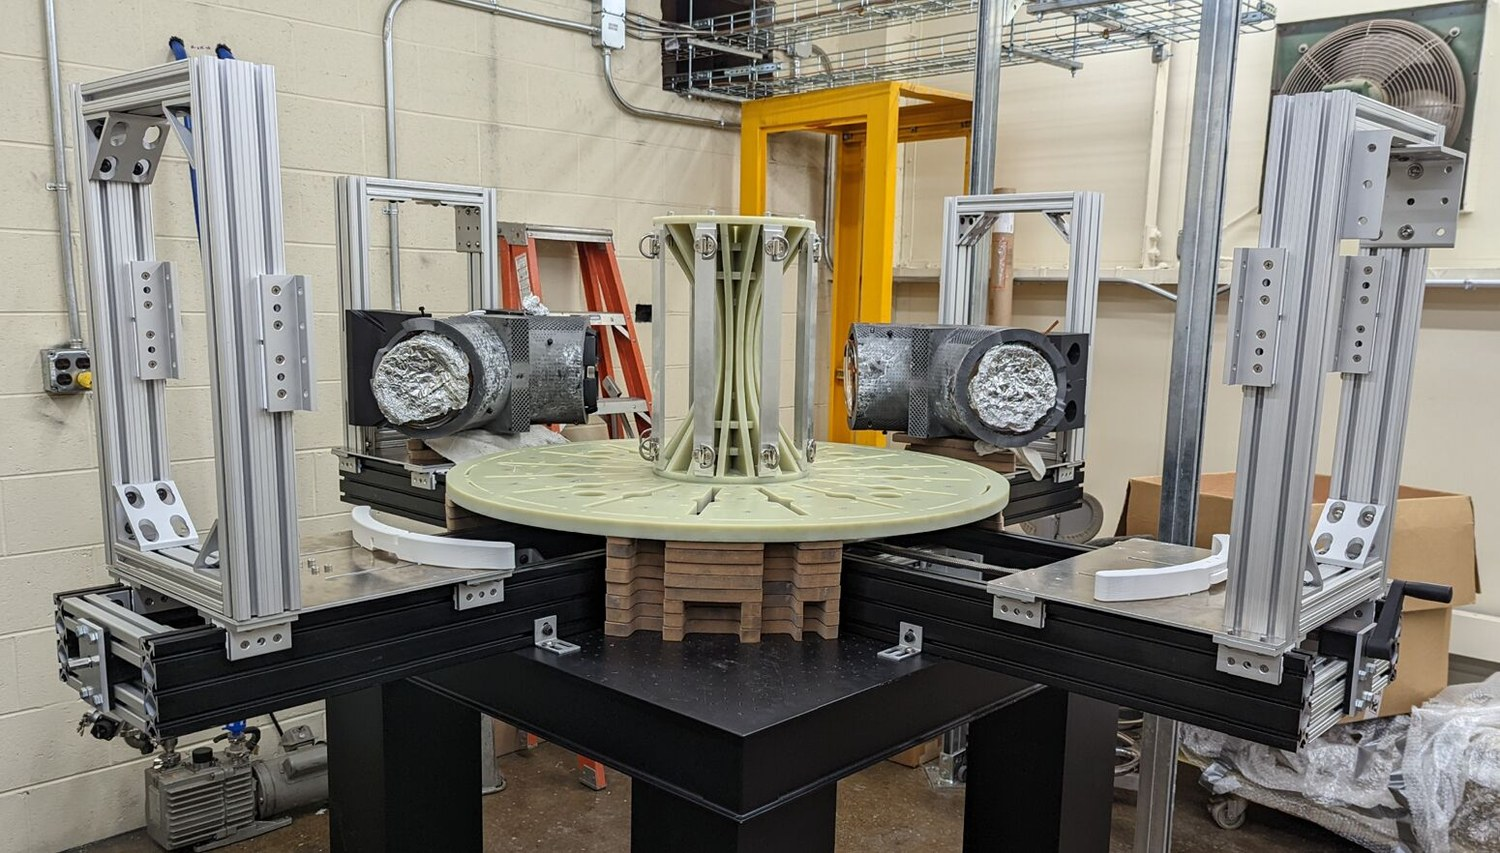
\includegraphics[width=0.72\textwidth]{../figures/aa_muse_stellarator.jpg}
\caption{仿星器不必靠复杂线圈：MUSE 用稀土永磁体拼出三维磁面，图中是它的装配现场。本节比较三种替代位形，这一条代表「不用等离子体电流也能有旋转变换」的现代做法。}
\label{fig:photo-appaa3}
\figsource{T. M. Qian 等（MUSE 团队），CC BY 4.0（Wikimedia Commons）}
\end{figure}

\section{旋转变换：仿星器为什么不需要等离子体电流}
\label{sec:app-aa-iota}

托卡马克的旋转变换来自等离子体电流：电流产生极向场，和环向场一起把磁力线拧成螺旋。
仿星器换了一条路：\textbf{用螺旋线圈把极向场直接「刻」进去}。两种做法都给出同一个几何量：
旋转变换 $\iota$（一圈环向走完，磁力线绕极向转了几圈），它与安全因子互为倒数：
\begin{equation}
\iota = \frac{1}{q}.
\label{eq:app-aa-iota}
\end{equation}
本附录的仿星器取边缘 $\iota/2\pi = 0.85$，于是 $q = 1.1765$。
\textbf{比 D1 的 $q_{95}=3$ 小得多}：仿星器的磁力线在极向绕得更快，
因为它的旋转变换是「按设计刻出来的」，可以取任意值。

托卡马克的 $q$ 剖面上还有一个有用的恒等式（附录 T 推过）：
\begin{equation}
s = \frac{r q'}{q} = 2 - \frac{2q_0}{q},
\label{eq:app-aa-shear}
\end{equation}
取 $q_0 = 1.05$、$q_{95} = 3.00$，得 $s = 1.3$。
\textbf{仿星器的 $s$ 可以设计成接近零（甚至为负）}。这叫「磁剪切优化」，
是仿星器能做而托卡马克做不到的事之一（托卡马克的 $s$ 由电流剖面绑死，
而电流剖面又由自举电流与电流驱动绑死）。

\begin{table}[htbp]
\centering
\small
\caption{旋转变换的两个来源。第三行是本节的重点：
\textbf{托卡马克的 $q$ 剖面是「电学量」，仿星器的 $\iota$ 剖面是「几何量」}——
前者只能间接调（改电流驱动），后者可以直接设计。}
\label{tab:app-aa-iota}
\begin{tabular}{p{3.4cm}p{3.2cm}p{3.2cm}p{3.3cm}}
\toprule
量 & D1 托卡马克 & 仿星器 & 含义 \\
\midrule
旋转变换 $\iota/2\pi$ & 由 $q$ 反推 & $0.85$ & 仿星器按设计取 \\
安全因子 $q$ & $q_{95} = 3.00$ & $1.1765$ & $q = 1/\iota$ \\
起始 $q_0$ & $1.05$ & 可自由设计 & 托卡马克受锯齿限制 \\
磁剪切 $s$ & $1.3$ & 可设计到 $\approx 0$ & 仿星器的独门手段 \\
\bottomrule
\end{tabular}

\end{table}

\begin{tip}{电流是「免费的旋转变换」，也是麻烦的来源}{tip-app-aa-iota}
托卡马克用等离子体电流造旋转变换，不用额外的线圈，听起来很划算。
但电流同时带来三件事：\textbf{欧姆加热与电流驱动要耗电}（附录 M）、
\textbf{电流剖面会自己演化到不稳定}（附录 V 的撕裂模与破裂）、
\textbf{电流不能无限大}（Greenwald 与 Troyan 极限）。
仿星器把这三件事一起消掉，代价是\textbf{线圈必须做成三维的}：
W7-X 的线圈有几十个不同形状的模块，装配公差是毫米级。
\textbf{工程复杂度换物理自由度}，这是仿星器的全部交易。
\end{tip}

{\footnotesize
\textbf{出处：}旋转变换与安全因子的关系、磁剪切恒等式参照 Helander
\emph{Theory of Stellarators}（2014，第 1、2 章）与附录 T 的推导。
W7-X 的 $\iota$ 剖面
量级取自 W7-X 装置手册。
}

\section{新经典输运：根号 eps 与 eps 有效值的二分之三次方}
\label{sec:app-aa-transport}

位形差别最直接的后果在输运上。托卡马克在香蕉区的新经典扩散系数按
\begin{equation}
\chi_{\mathrm{ban}} \propto \sqrt{\varepsilon}\,\chi_{\mathrm{PS}}
\label{eq:app-aa-sqeps}
\end{equation}
放大（$\chi_{\mathrm{PS}}$ 是平板值），D1 的 $\sqrt{\varepsilon} = 0.56796$。
仿星器没有轴对称，粒子轨道会\textbf{漂出磁面}，损失尺度不再由 $\varepsilon$ 而由一个更小的
「有效纹波」$\varepsilon_{\mathrm{eff}}$ 决定，且在 $1/\nu$ 区（碰撞很少时）按
\begin{equation}
\chi_{1/\nu} \propto \varepsilon_{\mathrm{eff}}^{3/2}\,\chi_{\mathrm{PS}}
\label{eq:app-aa-eff32}
\end{equation}
放大。优化后的仿星器取 $\varepsilon_{\mathrm{eff}} = 0.013$，
只有几何 $\varepsilon = 0.096364$ 的
\begin{equation}
\frac{\varepsilon_{\mathrm{eff}}}{\varepsilon} = 0.13491,
\label{eq:app-aa-effratio}
\end{equation}
于是 $\varepsilon_{\mathrm{eff}}^{3/2} = 0.00148223$。

把两个几何因子放在一起看：$\sqrt{\varepsilon_{D1}}/\varepsilon_{\mathrm{eff}}^{3/2}
= 383.181$。\textbf{但这个比值不能直接读成「仿星器输运好 383 倍」}。
两者处在不同的碰撞率区间，$\nu$ 的依赖方向正好相反：
托卡马克香蕉区的输运随碰撞率\textbf{上升}，仿星器的 $1/\nu$ 区随碰撞率\textbf{下降}。
所以仿星器有一个反直觉的结论：

\begin{equation}
\chi_{1/\nu} \propto \frac{1}{\nu}
\quad\Longrightarrow\quad
\text{温度越高（}\nu\text{ 越小）},\ \text{新经典损失越大}.
\label{eq:app-aa-1nu}
\end{equation}

\begin{table}[htbp]
\centering
\small
\caption{新经典输运的几何因子。最后一行是本附录最想提醒的一句：
\textbf{两个数处在不同物理区间时，除出来的倍数没有意义}——要先把区间对齐再比。}
\label{tab:app-aa-transport}
\begin{tabular}{p{3.4cm}p{3.2cm}p{3.2cm}p{3.3cm}}
\toprule
量 & 数值 & 由什么决定 & 含义 \\
\midrule
$\sqrt{\varepsilon_{D1}}$ & $0.56796$ & 托卡马克几何 & 香蕉区放大因子 \\
$\varepsilon_{\mathrm{eff}}$ & $0.013$ & 位形优化 & 声明值（优化位形） \\
$\varepsilon_{\mathrm{eff}}/\varepsilon$ & $0.13491$ & 优化品质 & 只有几何值的 $13.5\%$ \\
$\varepsilon_{\mathrm{eff}}^{3/2}$ & $0.00148223$ & $1/\nu$ 区 & 仿星器的几何因子 \\
两个因子的比 & $383.181$ & 不同区间 & \textbf{不可直接比较} \\
\bottomrule
\end{tabular}

\end{table}

\begin{tip}{不同区间的数不能直接相除}{tip-app-aa-eps}
看到 $\sqrt{\varepsilon}$ 与 $\varepsilon_{\mathrm{eff}}^{3/2}$ 都是「几何因子」，
很容易直接相除得到「好 $383$ 倍」。但这两个因子属于不同碰撞率区间：
香蕉区与 $1/\nu$ 区对 $\nu$ 的依赖方向相反，相等点在哪里取决于温度与密度。
\textbf{做任何跨位形的比较之前，先问一句「它们在同一个区间吗」}。
\end{tip}

{\footnotesize
\textbf{出处：}香蕉区 $\sqrt{\varepsilon}$ 输运参照 Wesson \emph{Tokamaks}（第 4 版，2011，第 2 章）。
仿星器 $1/\nu$ 区与有效纹波 $\varepsilon_{\mathrm{eff}}$ 的引入参照 Helander
\emph{Theory of Stellarators}（2014，第 3、4 章）。
}

\section{球形托卡马克：高比压与中心柱的空间代价}
\label{sec:app-aa-st}

球形托卡马克的想法很直接：把 $A$ 压到接近 $1$，$\varepsilon$ 就接近 $1$，
高 $\beta$ 与高自举电流份额随之而来。本附录的球形托卡马克取 $A=1.5$，
比压 $\beta = 4.027\%$，是 D1 的
\begin{equation}
\frac{\beta_{\mathrm{ST}}}{\beta_{D1}} = 3.0553
\end{equation}
倍。极向场由环向电流产生，边缘极向场为
\begin{equation}
B_p = \frac{\mu_0 I_p}{2\pi a} = 0.64516\ \mathrm{T},
\qquad
\beta_p = \frac{2\mu_0 p}{B_p^2} = 0.096742,
\label{eq:app-aa-bp}
\end{equation}
于是自举电流份额的量级（$C_{bs}$ 取 $1$）：
\begin{equation}
f_{bs} \approx C_{bs}\sqrt{\varepsilon}\,\beta_p = 0.078989.
\label{eq:app-aa-fbs}
\end{equation}
$7.9\%$ 看起来不大，但要与托卡马克的典型值（几个百分点）比。
\textbf{球形托卡马克能在没有电流驱动的条件下维持更大份额的电流}，
这就是「稳态运行更容易」的物理来源。

代价在几何上，而且可以精确算出来。中心柱能占的空间是
\begin{equation}
R - a,
\label{eq:app-aa-space}
\end{equation}
D1 有 $R-a = 4.2\ \mathrm{m}$，而附录 Z 算出中子屏蔽需要 $2.0723\ \mathrm{m}$。
\textbf{放得下}。球形托卡马克只有 $R-a = 0.31\ \mathrm{m}$，
比屏蔽需求小 $6.6848$ 倍。\textbf{放不下}。

\begin{table}[htbp]
\centering
\small
\caption{球形托卡马克的账。最后两行是本节的核心：
\textbf{物理上更优（高 $\beta$、高自举份额），工程上却被 $0.31\ \mathrm{m}$ 卡死}——
中心柱放不下中子屏蔽，也放不下足够的氚增殖区。}
\label{tab:app-aa-st}
\begin{tabular}{p{3.6cm}p{3.0cm}p{3.0cm}p{3.2cm}}
\toprule
量 & D1 托卡马克 & 球形托卡马克 & 含义 \\
\midrule
比压 $\beta$ & $1.318\%$ & $4.027\%$ & 高 $3.0553$ 倍 \\
边缘极向场 $B_p$ & --- & $0.64516\ \mathrm{T}$ & $\mu_0I_p/(2\pi a)$ \\
极向比压 $\beta_p$ & --- & $0.096742$ & 声明 $I_p = 2\ \mathrm{MA}$ \\
自举份额 $f_{bs}$ & 几个 $\%$ & $0.078989$ & $C_{bs}\sqrt{\varepsilon}\beta_p$ \\
中心柱空间 $R-a$ & $4.2\ \mathrm{m}$ & $0.31\ \mathrm{m}$ & 屏蔽需要 $2.0723\ \mathrm{m}$ \\
与屏蔽需求之比 & 放得下 & 少 $6.6848$ 倍 & \textbf{堆用不了} \\
\bottomrule
\end{tabular}

\end{table}

\begin{tip}{物理的优化可能被几何一票否决}{tip-app-aa-st}
球形托卡马克的每一条物理指标都比托卡马克漂亮：$\beta$ 高 $3.0553$ 倍、
自举份额大、装置紧凑便宜。但 $R-a = 0.31\ \mathrm{m}$ 这一个数就把「堆」的可能性关掉了。
中子屏蔽要 $2.0723\ \mathrm{m}$（附录 Z），$0.31$ 连零头都不够。
\textbf{所以球形托卡马克的定位是「紧凑中子源与研究装置」，不是发电堆}。
教训：做方案评价时，除了算物理指标，一定还要算\textbf{空间、屏蔽与维护通道}这三个「几何硬约束」。
\end{tip}

{\footnotesize
\textbf{出处：}球形托卡马克的高 $\beta$ 与自举电流份额参照 Peng \& Strickler
（1986）\emph{Nucl.\ Fusion} \textbf{26}, 769 与 NSTX 装置手册。
自举份额的标度形式参照 Wesson（2011，第 2 章）。
屏蔽厚度沿用附录 Z 的 $2.0723\ \mathrm{m}$。
}

\begin{figure}[htbp]
\centering
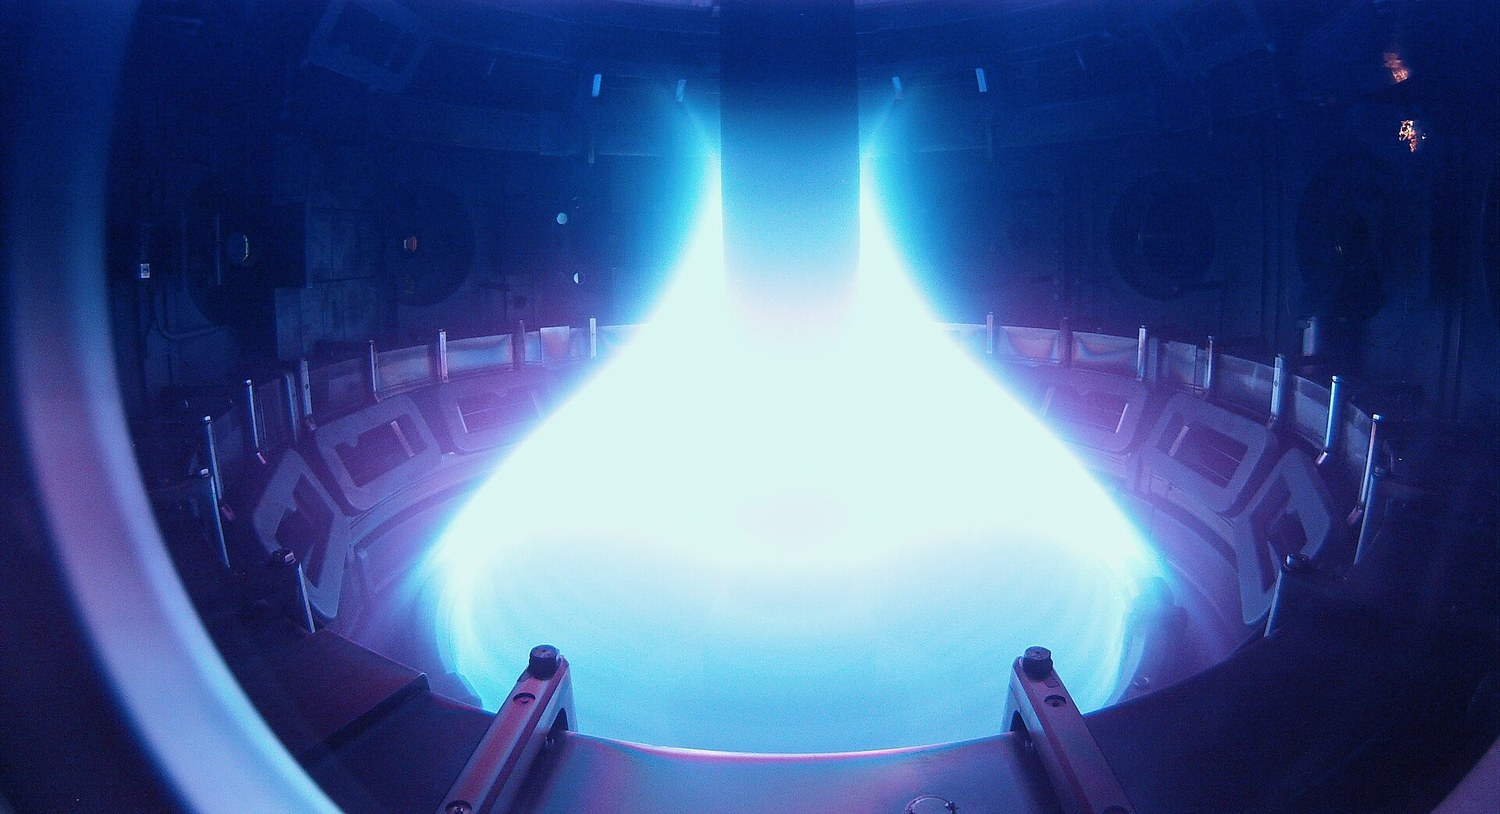
\includegraphics[width=0.72\textwidth]{../figures/mast_tokamak.jpg}
\caption{MAST 球形托卡马克：中心柱换来的高比压。球形托卡马克把环径比压到接近 1：同样磁场下能装更高的比压，代价是中心柱占掉了本来可以放等离子体的空间。本节算的 $\beta_N$ 与中心柱空间账，就是这台装置与常规托卡马克的分水岭。}
\label{fig:photo-appa2}
\figsource{Eye Steel Film，CC BY 2.0（Wikimedia Commons）}
\end{figure}

\section{场反位形：比压等于一，代价是稳定性}
\label{sec:app-aa-frc}

场反位形（FRC）把「省」做到底：不要环向场，只用一个\textbf{反平行的环向电流}
（内部电流与外部电流方向相反）把磁场闭合成一个封闭的位形。
位形内部的总磁场为零，压力全部由外部磁场顶住：
\begin{equation}
p = \frac{B_{\mathrm{ext}}^2}{2\mu_0},
\label{eq:app-aa-frcp}
\end{equation}
取 $B_{\mathrm{ext}} = 0.5\ \mathrm{T}$，得 $p = 99472\ \mathrm{Pa}$。
这就是 $\beta = 1$ 的含义：\textbf{磁压全部用来装等离子体，一点不剩}。
在 $T = 1.0\ \mathrm{keV}$ 下对应的密度是
\begin{equation}
n = \frac{p}{k_BT} = 6.2085\times10^{20}\ \mathrm{m^{-3}},
\label{eq:app-aa-frcn}
\end{equation}
维持这个位形需要的反平行电流为
\begin{equation}
I = \frac{2\pi r_s B_{\mathrm{ext}}}{\mu_0} = 1\times10^{6}\ \mathrm{A} = 1\ \mathrm{MA},
\label{eq:app-aa-frci}
\end{equation}
长细比 $L/(2r_s) = 10$。作为对照：\textbf{D1 的环向电流 $9\ \mathrm{MA}$ 全部用来产生旋转变换，
而 FRC 的 $1\ \mathrm{MA}$ 只用来维持自己的位形}。两者不是同一类量。

代价是稳定性。FRC 是\textbf{没有磁剪切}的位形（内部 $q\to0$），
所以理想 MHD 的结论是它本该被 $n=1$ 倾斜模撕掉；
实验上能活下来是因为动理学效应（大回旋半径、离子束）把模稳住了。
本附录不引入任何阈值数字（与附录 V 的口径一致），只给出这条边界：

\begin{equation}
\beta = 1,\qquad q \to 0,\qquad \text{稳定性靠动理学而不是磁剪切}.
\label{eq:app-aa-frclimit}
\end{equation}

\begin{table}[htbp]
\centering
\small
\caption{场反位形的全部账。最后一行是刻意的：
\textbf{本附录不给倾斜模的阈值数字}——那需要动理学计算，超出本附录的边界
（与附录 W「明说给不出阈值」同一口径）。}
\label{tab:app-aa-frc}
\begin{tabular}{p{3.4cm}p{3.2cm}p{3.2cm}p{3.3cm}}
\toprule
量 & 数值 & 由什么决定 & 含义 \\
\midrule
外部磁场 $B_{\mathrm{ext}}$ & $0.5\ \mathrm{T}$ & 声明值 & 位形全靠它 \\
压力 $p$ & $99472\ \mathrm{Pa}$ & $B^2/(2\mu_0)$ & $\beta = 1$ \\
密度（$1.0\ \mathrm{keV}$） & $6.2085\times10^{20}\ \mathrm{m^{-3}}$ & $p/k_BT$ & 比 D1 高六倍 \\
反平行电流 & $1\ \mathrm{MA}$ & $2\pi r_sB/\mu_0$ & 只维持位形 \\
长细比 & $10$ & $L/(2r_s)$ & 细长的雪茄 \\
稳定性 & 靠动理学 & 无磁剪切 & \textbf{不给阈值} \\
\bottomrule
\end{tabular}

\end{table}

\begin{tip}{比压等于一不是「极限」，是「定义」}{tip-app-aa-frc}
托卡马克里 $\beta$ 是「磁压用了多少」，所以有上限（Troyon 极限，附录 M）；
FRC 里 $\beta=1$ 是\textbf{位形的定义}：内部磁场为零、压力全部由外部场顶住。
所以看到「FRC 的 $\beta=1$」不要读成「它比 D1 的 $\beta$ 强 $75.87$ 倍」：
两者根本不是同一个优化问题。\textbf{同一个符号在不同位形里可以是完全不同的东西}。
\end{tip}

{\footnotesize
\textbf{出处：}FRC 的压力平衡与反平行电流图像参照 Tuszewski（1988）
\emph{Nucl.\ Fusion} \textbf{28}, 2033。
$n=1$ 倾斜模与动理学稳定机制的量级参照
Steinhauer（2011）\emph{Phys.\ Plasmas} \textbf{18}, 070501。本节数字由
\texttt{tools/\allowbreak{}calc/\allowbreak{}appAA\_calc.py} 复算。
}

\section{定标与三重积：替代位形离点火有多远}
\label{sec:app-aa-scaling}

最后一步是把三种位形放进同一个「约束语言」里。托卡马克用 IPB98(y,2)（附录 S），
仿星器有它自己的定标 ISS04：
\begin{equation}
\tau_E^{\mathrm{ISS04}} = 0.134\,a^{2.28}R^{0.64}P^{-0.61}
n^{0.54}B^{0.84}\iota^{0.41},
\label{eq:app-aa-iss04}
\end{equation}
（单位：$\mathrm{m}$、$\mathrm{MW}$、$10^{19}\ \mathrm{m^{-3}}$、$\mathrm{T}$，$\iota$ 取边缘 $\iota/2\pi$）。
代入本附录的仿星器参数（$a = 0.53$、$R = 5.5$、$P = 10\ \mathrm{MW}$、$n = 8\times10^{19}$、
$B = 2.5$、$\iota = 0.85$）：
\begin{equation}
\tau_E^{\mathrm{ISS04}} = 0.142983\ \mathrm{s},
\label{eq:app-aa-tauE}
\end{equation}
而 D1 的 IPB98 值是 $2.4762\ \mathrm{s}$，两者之比
\begin{equation}
\frac{\tau_E^{\mathrm{ISS04}}}{\tau_E^{\mathrm{IPB98}}(D1)} = 0.057743
\label{eq:app-aa-ratio}
\end{equation}
\textbf{这个比值不是「仿星器差 17 倍」}。两台装置的尺寸与功率完全不同。
它真正说明的是：W7-X 量级是一个\textbf{研究装置}，把它的参数代进三重积：
\begin{equation}
n\,T\,\tau_E = 2.28774\times10^{19}
\quad\text{vs}\quad
\text{点火阈值 } 3.1\times10^{21},
\label{eq:app-aa-triple}
\end{equation}
还差 $135.51$ 倍。作为对照，附录 U 的 D1 已经站在点火门槛附近。
这也解释了为什么仿星器路线的下一步不是「把 W7-X 做大」，
而是\textbf{先把 $\iota$、$B$ 与 $P$ 这几个旋钮的方向找对}：
式 \eqref{eq:app-aa-iss04} 里 $\iota$ 的指数是 $+0.41$，
把 $\iota/2\pi$ 从 $0.85$ 提到 $1.00$ 只把 $\tau_E$ 提高 $1.0689$ 倍（$+6.8903\%$），
而 $B$ 的指数是 $+0.84$。\textbf{磁场比旋转变换值更值得投入}。

\begin{table}[htbp]
\centering
\small
\caption{把仿星器放进三重积语言。第四行是与 D1（$2.4762\ \mathrm{s}$）的对照，
但\textbf{两台装置不可直接比}——真正可比的量是最后一行与阈值的距离。}
\label{tab:app-aa-scaling}
\begin{tabular}{p{3.4cm}p{3.2cm}p{3.2cm}p{3.3cm}}
\toprule
量 & 数值 & 由什么决定 & 含义 \\
\midrule
ISS04 系数 & $0.134$ & 声明值 & 仿星器定标 \\
$\iota$ 的指数 & $+0.41$ & ISS04 & $\iota\uparrow$ 约束改善慢 \\
$B$ 的指数 & $+0.84$ & ISS04 & 磁场更有效 \\
$\tau_E^{\mathrm{ISS04}}$ & $0.142983\ \mathrm{s}$ & 式 \eqref{eq:app-aa-iss04} & 研究装置量级 \\
三重积 & $2.28774\times10^{19}$ & $nT\tau_E$ & 差 $135.51$ 倍 \\
\bottomrule
\end{tabular}

\end{table}

\begin{tip}{定标律是「代理」，不是物理}{tip-app-aa-honest}
ISS04 有 $6$ 个自由指数、$1$ 个前置系数，全部是拟合出来的。
它能告诉你\textbf{方向}（$B$ 比 $\iota$ 值更值得投），但不能告诉你\textbf{机制}。
所以本附录用它只做一件事：把三种位形放进同一个语言里比较。
与附录 S 对 IPB98(y,2) 的处理完全一致：\textbf{同一个经验定标，
在经验范围内用，超出范围就明说不能用}。这也是本附录对「借鉴经典教材」这条长期目标的
一贯做法：借结论、借结构、借题型，但把每一个数字都用自己的脚本在声明的参数上现算。
\end{tip}

{\footnotesize
\textbf{出处：}ISS04 定标参照 Yamada 等（2005）\emph{Nucl.\ Fusion} \textbf{45}, 1684，三重积阈值与点火条件沿用附录 U 的口径。
IPB98(y,2) 的 D1 值来自附录 S。
}

\section{估算练习}
\label{sec:app-aa-problems}

\textbf{练习 1} 球形托卡马克的中心柱能占多少空间？与附录 Z 算出的中子屏蔽厚度
$2.0723\ \mathrm{m}$ 相比差多少倍？这说明了什么？

\textbf{练习 2} 若把仿星器的边缘 $\iota/2\pi$ 从 $0.85$ 提高到 $1.00$，
按 ISS04 定标 $\tau_E$ 变成多少倍？涨幅是多少？

\textbf{练习 3} 若把 FRC 的外部磁场从 $0.5\ \mathrm{T}$ 加倍到 $1.0\ \mathrm{T}$，
$\beta=1$ 对应的压力与密度各变成多少？（写出倍数与数值。）

\textbf{练习 4} 球形托卡马克与 D1 的比压之比是多少？为什么它们的 $\beta_N$ 反而差不多？

\textbf{练习 5} 若 $\varepsilon_{\mathrm{eff}}$ 从 $0.013$ 降到 $0.0065$（优化更好），
$\varepsilon_{\mathrm{eff}}^{3/2}$ 变成原来的多少倍？

\textbf{练习 6} 若把球形托卡马克的环向场从 $1.0\ \mathrm{T}$ 提到 $1.5\ \mathrm{T}$
（密度与温度不变），比压变成多少？$\beta_N$ 变成多少？

\textbf{解答 1} $R-a = 0.93-0.62 = 0.31\ \mathrm{m}$，
比 $2.0723\ \mathrm{m}$ 少 $6.6848$ 倍。\textbf{要点}：中心柱放不下中子屏蔽，
所以球形托卡马克只能做紧凑中子源或研究装置，不能直接当发电堆。
\textbf{物理指标再漂亮，也可能被一个几何数一票否决}。

\textbf{解答 2} $\tau_E \propto \iota^{0.41}$，所以倍数为
$(1.00/0.85)^{0.41} = 1.0689$，涨幅 $6.8903\%$。
\textbf{要点}：与 $B$ 的指数 $0.84$ 比，$\iota$ 的杠杆小一半。
\textbf{调参数之前先看指数}。

\textbf{解答 3} $p = B^2/(2\mu_0) \propto B^2$，所以压力与密度都变成 $4$ 倍：
$p = 3.9789\times10^{5}\ \mathrm{Pa}$、$n = 2.4834\times10^{21}\ \mathrm{m^{-3}}$。
\textbf{要点}：$\beta=1$ 位形的密度由 $B^2$ 决定，所以「提高磁场」在 FRC 上是
\textbf{直接把密度翻两番}的手段。这也是它比托卡马克更依赖强磁场的道理。

\textbf{解答 4} $\beta_{\mathrm{ST}}/\beta_{D1} = 3.0553$；
而 $\beta_N$ 分别是 $1.2483$ 与 $1.5523$，差不多。
\textbf{要点}：$\beta_N$ 把 $a$、$B$、$I_p$ 三个「装置尺度」除掉了，
所以它才是跨装置可比的量；$\beta$ 只反映「磁压用了多少」，
装置越小越容易做高（同样的 $B$ 下，$p$ 相同而 $B$ 更低时 $\beta$ 更大）。

\textbf{解答 5} $\varepsilon_{\mathrm{eff}}^{3/2} \propto \varepsilon_{\mathrm{eff}}^{1.5}$，
减半后变成 $0.5^{1.5} = 0.353553$ 倍。\textbf{要点}：$1/\nu$ 输运对
$\varepsilon_{\mathrm{eff}}$ 是 $3/2$ 次方，所以\textbf{把有效纹波压小一点点，
收益是超线性的}。这就是位形优化（准对称、准等动）值得投入的原因。

\textbf{解答 6} $\beta \propto 1/B^2$，所以 $\beta = 4.027\%/2.25 = 1.79\%$；
$\beta_N \propto \beta B$，于是 $\beta_N = 1.2483\times(1.5/1.0)/2.25 = 0.8322$。
\textbf{要点}：提高磁场会把 $\beta$ 压下去，但 $\beta_N$ 也一起掉。
\textbf{「提高磁场」与「提高比压」是两条不同的路}，前者提高密度上限，
后者提高磁场的利用率。

\section{来源、分级与版权说明}
\label{sec:app-aa-source}

\begingroup\small
本附录按难度分三档。AA.1 与 AA.2 是几何与旋转变换（读完应当能说清「仿星器为什么不需要电流」）。
AA.3 与 AA.4 是两个位形的核心代价（读完应当能独立算出有效纹波因子与中心柱空间账）。
AA.5 与 AA.6 是极端位形与定标（读完应当能把三种位形放进同一个语言里比较）。
练习 1--6 都只需要本附录的公式与表，不需要查外部数据。

\begin{table}[htbp]
\centering
\small
\caption{本附录的借鉴来源与对应位置。只借鉴物理结论、公式形式与题型；
全部数值、表格与文字自拟并由仓库脚本复算。}
\label{tab:app-aa-source}
\begin{tabular}{p{3.4cm}p{5.6cm}p{3.6cm}}
\toprule
本附录内容 & 借鉴来源 & 在本书里的位置 \\
\midrule
位形分类与比压定义 &
Freidberg \emph{Ideal Magnetohydrodynamics}（1987）第 1 章；Wesson \emph{Tokamaks}（第 4 版，2011）第 1 章 &
附录 S、本附录 AA.1 \\
旋转变换、磁剪切与位形优化 &
Helander \emph{Theory of Stellarators}（2014）第 1、2 章 &
附录 T、本附录 AA.2 \\
$1/\nu$ 输运与有效纹波 &
Helander（2014）第 3、4 章 &
本附录 AA.3 \\
球形托卡马克与自举电流 &
Peng \& Strickler（1986）\emph{Nucl.\ Fusion} \textbf{26}, 769；NSTX 装置手册 &
附录 M 的自举电流、本附录 AA.4 \\
场反位形与倾斜模 &
Tuszewski（1988）\emph{Nucl.\ Fusion} \textbf{28}, 2033；Steinhauer（2011）\emph{Phys.\ Plasmas} \textbf{18}, 070501 &
本附录 AA.5 \\
ISS04 约束定标 &
Yamada 等（2005）\emph{Nucl.\ Fusion} \textbf{45}, 1684 &
附录 S 的 IPB98、本附录 AA.6 \\
\bottomrule
\end{tabular}

\end{table}

版权与复现口径，四条：第一，\textbf{不复制}任何教材或论文的表格数值，
表 \ref{tab:app-aa-map} 到表 \ref{tab:app-aa-source} 的每一个数字都由
\texttt{tools/\allowbreak{}calc/\allowbreak{}appAA\_calc.py} 在给定参数上现算；

第二，\textbf{不复制}原书的题面与解答文字，
练习 1--6 的题目与解答均为本书自拟；

第三，\textbf{不复制}无法核验的 DOI 编号，
一律只给书名、作者、年份、卷期页；

第四，\textbf{不复制}任何未经复算的「精确值」。
凡本附录引入的\textbf{声明值}（三种位形的装置级参数、球形托卡马克的 $I_p = 2\ \mathrm{MA}$、
仿星器的 $P = 10\ \mathrm{MW}$ 与 $\varepsilon_{\mathrm{eff}} = 0.013$、
FRC 的 $B_{\mathrm{ext}} = 0.5\ \mathrm{T}$ 与 $r_s = 0.4\ \mathrm{m}$、
自举系数 $C_{bs} = 1$、ISS04 的系数与六个指数）都在正文里写明是量级值或拟合系数，
不假装精确。
\endgroup
